\section{Results and discussion} \label{Results-and-discussion}

\subsection{Excess reactivity}

The excess reactivity $\rho$$_e$ is calculated at zero burnup (steady state 
calculation), when all control rods (CRs) are fully withdrawn. The $\rho_e$ for $^{233}$U, 
reactor-grade Pu, and TRU used as initial fissile material are listed in Table~\ref{tab:excess}.
The previously studied $^{233}$U case recorded the maximum reactivity
during 60 effective full-power years (EFPY) of reactor operation to be 
$4.27\pm0.01$ $\$$ (see Figure~\ref{fig:keff_25}).
The proposed reactivity control system must compensate such reactivity at startup and during burnup.
\begin{figure}
	\centering
	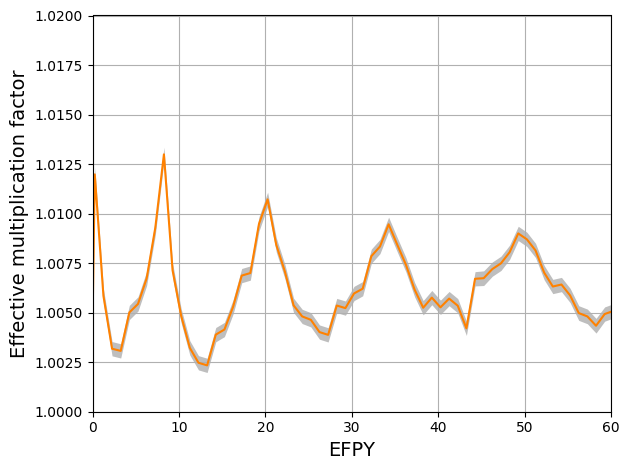
\includegraphics[width=\textwidth]{keff_25.png}
	\vspace{-0.5in}
	\caption{Uncontrolled effective multiplication factor during 60 EFPY of reactor operation including periodic fissile material insertion (confidence interval $\pm\sigma$ is shaded) \cite{ashraf2020whole}.} 
	\label{fig:keff_25}
\end{figure}

\begin{table}  %[!hb]
	\caption{The excess reactivity for the SD-TMSR core with different initial fissile materials.}
	\vspace{0.1in}
	\begin{tabularx}{\textwidth}{p{3cm} s s s}
		\hline
		Initial fissile materials       				&  $^{233}$U & reactor-grade Pu&  TRU \\
		\hline
		$\rho_e$					& $1.65\pm0.04$ $\$$ & $4.11\pm0.02$ $\$$ & $15.38\pm0.04$ $\$$ \\
		\hline
	\end{tabularx}
	\label{tab:excess}
\end{table}

\subsection{Control rod parameters}

The control rod parameters including control rod worth (CRW), interference 
between CR clusters, and integral and differential control rod worths are 
described in this part. 
Table~\ref{tab:worth} shows calculated CRW, the amplification 
factor (A$_{CRi}$), and the type of interference for six different 
absorbers.

\begin{sidewaystable}
	\fontsize{5}{7}\selectfont
	\centering
	\caption{The control rod worth and shadowing effect for different CR 
	materials.}
	\vspace{1ex}
	\begin{tabularx}{\textwidth}{|p{1.8cm}|p{0.56cm}|p{0.5cm}|p{0.49cm}|p{0.56cm}|p{0.5cm}|p{0.49cm}| 
	p{0.56cm}|p{0.5cm}|p{0.49cm}|p{0.56cm}|p{0.5cm}|p{0.49cm}| 
	p{0.56cm}|p{0.5cm}|p{0.49cm}|p{0.56cm}|p{0.5cm}|p{0.49cm}|}
		\hline
		\multirow{2}{*}{Control Rod group}		& 
		\multicolumn{3}{c|}{Nat. B$_4$C} & \multicolumn{3}{c|}{B$_4$C-90}   	&\multicolumn{3}{c|}{HfB$_2$}	
		&\multicolumn{3}{c|}{HfH$_{1.62}$} 
		&\multicolumn{3}{c|}{Gd$_2$O$_3$}	& 	
		\multicolumn{3}{c|}{Eu$_2$O$_3$} \\
		\cline{2-19}
		& $\Delta\rho$$_{CRi}$  [\$]  &A$_{CRi}$	& Inter\-ference
		& $\Delta\rho$$_{CRi}$  [\$]  &A$_{CRi}$	& Inter\-ference	
		&$\Delta\rho$$_{CRi}$ [\$]  &A$_{CRi}$	& Inter\-ference	
		&$\Delta\rho$$_{CRi}$ [\$]	&A$_{CRi}$	& Inter\-ference	
		&$\Delta\rho$$_{CRi}$ [\$]	&A$_{CRi}$	& Inter\-ference	
		&$\Delta\rho$$_{CRi}$ [\$]	&A$_{CRi}$  &	Inter\-ference \\
		\hline                   
		All control rods      &  $42.04\pm0.60$	&	&		& $48.19\pm0.68$   &	&	
		&$40.40\pm0.41$	&	&	&$37.96\pm0.36$	&	&	&$33.70\pm0.40$	&	
		&	&$42.39\pm0.48$	& &	 \\
		\hline 
		CSD 		 & $22.32\pm0.20$ 	& $1.24\pm0.01$	&	$\star$				& $25.50\pm0.23$   &$1.24\pm0.01$	&$\star$	&$21.90\pm0.17$	&$1.10\pm0.01$	&$\star$	&$20.62\pm0.34$	&$1.10\pm0.01$	&$\star$	&$18.48\pm0.25$	&$1.17\pm0.01$	&$\star$	&$22.96\pm0.18$	&$1.20\pm0.01$ &$\star$ \\
		\hline 
		SSD		   & $14.27\pm0.10$ 	&$1.38\pm0.02$	&	$\star$	&$16.39\pm0.11$ &$1.38\pm0.02$	&$\star$	&$14.27\pm0.21$	&$1.29\pm0.01$	&$\star$	&$13.23\pm0.18$	&$1.30\pm0.06$	&$\star$	&$12.00\pm0.20$	&$1.26\pm0.01$	&$\star$	&$14.58\pm0.11$	&$1.30\pm0.02$	&$\star$ \\
		\hline 
		CSD inner ring   &  $16.80\pm0.02$	&$1.50\pm0.01$	&$\star$ &  $18.42\pm0.05$  &$1.60\pm0.04$	&$\star$		&$16.29\pm0.29$	&$1.48\pm0.02$	&$\star$	&$15.50\pm0.17$	& $1.46\pm0.01$ &$\star$	&$14.12\pm0.07$	&$1.39\pm0.01$	&$\star$	&$16.92\pm0.13$	&$1.50\pm0.01$	 &$\star$\\
		\hline 
		CSD outer ring            &  $2.16\pm0.02$	&$3.11\pm0.06$	&	$\star$    &$2.26\pm0.02$ &$4.21\pm0.07$	&$\star$	&$2.10\pm0.06$	&$3.11\pm0.10$&$\star$	&$1.85\pm0.07$	&$3.24\pm0.06$	&$\star$	&$1.80\pm0.10$	&$2.54\pm0.14$	&$\star$	&$2.14\pm0.05$	&$3.20\pm0.05$	 &$\star$	\\
		\hline 
		CSD2			 &  $2.11\pm0.03$	&$3.00\pm0.08$	&	$\star$				& $2.25\pm0.04$   &$3.69\pm0.16$	&$\star$	&$2.24\pm0.05$	&$2.42\pm0.10$	&$\star$	&$2.00\pm0.10$	&$2.68\pm0.03$	&$\star$	&$1.80\pm0.10$	&$2.55\pm0.20$	&$\star$	&$2.19\pm0.12$	&$2.90\pm0.08$	&$\star$ \\
		\hline 
		CSD9			 &  $0.06\pm0.01$	&$15.16\pm0.10$	&	$\star$$\star$				& $0.15\pm0.04$   & $10.53\pm0.01$	&$\star$$\star$	&$0.10\pm0.05$	&$5.10\pm0.05$	&$\star$	&$0.05\pm0.01$	&$16.40\pm0.10$	&$\star$$\star$	&$0.09\pm0.07$	&$5.55\pm0.20$	&$\star$$\star$	&$0.07\pm0.05$	&$14.00\pm0.10$	&$\star$$\star$ \\ 
		\hline
		SSD1		 &  $3.95\pm0.05$	&$1.31\pm0.01$	&	$\star$		& $4.18\pm0.07$   &$1.59\pm0.08$	&$\star$	&$3.95\pm0.13$	&$1.30\pm0.07$	&$\star$	&$3.59\pm0.03$	&$1.49\pm0.01$	&$\star$	&$3.45\pm0.12$	&$1.40\pm0.08$	&$\star$	&$3.91\pm0.06$	&$1.40\pm0.01$&$\star$ \\
		\hline 
		SSD4		 &  $0.59\pm0.08$	& $9.52\pm0.10$	&	$\star$$\star$		&  $0.57\pm0.09$  &$7.84\pm0.15$	&$\star$$\star$	&$0.63\pm0.06$	&$4.40\pm0.10$	&$\star$	&$1.00\pm0.05$	&$2.51\pm0.16$	&$\star$	&$0.60\pm0.80$	&$3.31\pm0.27$	&$\star$	&$0.60\pm0.08$	&$5.10\pm0.28$	&$\star$$\star$ \\
		\hline
	\end{tabularx}
	\begin{tablenotes}
		\tiny
		\item  $\star$  anti-shadowing effects observed
		\item  $\star$$\star$ strong anti-shadowing effects observed
	\end{tablenotes}
	\label{tab:worth}
\end{sidewaystable}

\subsubsection{CRW} \label{CR_worth}

Among the absorbers investigated, the total worth of all CRs extends from $33.7\pm0.4$ $\$$ to $48.19\pm0.68$ 
$\$$ (the first row in Table~\ref{tab:worth}). B$_4$C-90 (boron enriched to 90\% $^{10}$B)
has the largest absorption ability, while Gd$_2$O$_3$ has the lowest 
absorption compared with the other absorbing materials in this study. This 
result agrees with macroscopic absorption cross section data 
\cite{guo2019optimized}. B$_4$C-90 has the highest macroscopic 
absorption cross section followed by Eu$_2$O$_3$, natural B$_4$C (Nat. B$_4$C), HfB$_2$, HfH$_{1.62}$, and 
finally Gd$_2$O$_3$. The CR material is being transmuted during 
operation; the effect of the fuel salt burnup on the CRW is neglected
herein and will be investigated and presented in Part II of this 
study.

The worth of the Control Safety Devices (CSD) clusters is $1.56$ times greater than 
the worth of the Shutdown Safety Devices (SSD) system for all absorbing materials. Either CSD or SSD 
clusters are able to shut down the reactor initially loaded by 
$^{233}$U and reactor-grade Pu regardless the absorbing material type.
However, only SSD clusters made of B$_4$C-90 are able to shut down the SD-TMSR 
initially loaded by transuranic (TRU) elements ($\rho_e$ is $15.38\pm0.04$ $\$$).
The reason for this is the much larger 
absorption cross section of $^{10}$B in the relatively soft neutron energy 
spectrum of the SD-TMSR core started with TRU \cite{ashraf2020Strategies}.

The inner ring of the CSD is located in the central zone of the SD-TMSR core 
(Figure~\ref{fig:core_25}), in which the volume ratio between molten salt and 
graphite is relatively small ($0.357$). Results show that the inner ring of the CSD has 
a worth almost equal to the worth of all other CRs together (SSD + CSD outer ring) regardless of 
the absorbing material type (see Table~\ref{tab:worth}). This happens because the absorption cross section
decreases with the energy of the incident neutron; for example, boron absorbs neutrons in the thermal spectrum much 
greater than in the fast spectrum.

In case of malfunction of other CR clusters (e.g., stuck in the upper 
position), the outer ring of the CSD will be able to compensate the excess reactivity of the core initially loaded by $^{233}$U.
Meanwhile, it will fail to compensate the excess 
reactivity of the core initially loaded by reactor-grade Pu and TRU elements.

We separately calculated the worth of CSD2, CSD9, SSD1, and SSD4 clusters (i.e. clusters located in the center and at the boundary between the core
zones, see Figure~\ref{fig:core_25}) to investigate the variation of CRW with the position in the inner core.
The CRW decreases in the direction of the outer core zone. The outer core zone 
has smaller moderator-to-fuel ratio ($0.86$) compared with the central zone 
($2.8$); consequently, the neutron energy spectrum is faster in the peripheral 
zone than in the center of the core degrading the CR's 
absorption ability in that region.

\subsubsection{Shutdown margin (SDM)}

The Shutdown Safety Devices (SSD) clusters are designed mainly for an emergency shutdown, thus it should 
provide the reactor core with sufficient negative reactivity. The 
shutdown margin (SDM) is calculated by equation~\ref{Equ:6}.
Table~\ref{tab:table2} summarizes the shutdown margins for the SD-TMSR core 
initially loaded with $^{233}$U, reactor-grade Pu, and TRU 
elements for different absorbing materials. All absorbing materials provide a sufficient positive
SDM for the SD-TMSR core that is initially loaded with 
$^{233}$U and reactor-grade Pu. However, the SDMs for the TRU case are 
negative or slightly positive (in B$_4$C-90 case); this makes the SSD clusters 
unreliable to shut down the reactor loaded with TRU.
As mentioned previously, the SSD clusters should 
provide a sufficient positive SDM.

\begin{table}  %[!hb]
	\caption{The SDMs for the SD-TMSR core for different absorbing materials.}
	\vspace{0.1in}
	\begin{tabularx}{\textwidth}{p{3cm} s s s}
		\hline
		Absorbing materials        				&  $^{233}$U & reactor-grade Pu&  TRU \\
		\hline
		Nat. B$_4$C					& $12.62\pm0.08$ $\$$ &$10.18\pm0.09$ $\$$ &$-1.12\pm0.08$ $\$$ \\
		B$_4$C-90                          & $14.74\pm0.09$ $\$$ & $12.28\pm0.12$ $\$$ & $ $ $ $ $1.01\pm0.09$ $\$$ \\
		Eu$_2$O$_3$                       &  $12.93\pm0.09$ $\$$    &  $10.47\pm0.12$ $\$$   &$-0.80\pm0.09$ $\$$\\
		HfB$_2$        				 &$12.62\pm0.24$ $\$$ &$10.16\pm0.26$ $\$$ &$-1.11\pm0.24$ $\$$   \\
		HfH$_{1.62}$							& $11.58\pm0.19$ $\$$ &$9.12\pm0.22$ $\$$ &$-2.15\pm0.19$ $\$$ \\
		Gd$_2$O$_3$	  		& $10.35\pm0.22$ $\$$ &$7.890\pm0.25$ $\$$& $-3.38\pm0.22$ $\$$\\
		\hline
	\end{tabularx}
	\label{tab:table2}
\end{table}

\subsubsection{Interference between CR systems}

The amplification factor (A$_{CRi}$) results show that the CSD, SSD, CSD inner 
ring, and SSD1 are slightly amplified due to the anti-shadowing effects. The 
anti-shadowing is observed when the combined rod worth is greater than the sum 
of the individual worths. The strongest anti-shadowing effect occurred in 
SSD4 and CSD9 clusters that are located at the boundary between the core zones 
with different moderator-to-fuel ratios (see Table~\ref{tab:worth}).
The obtained results emphasize that no relation exists between the absorbing
material type and the interference between the CR clusters
(i.e. the A$_{CRi}$).

Insertion of the CR affects the neutron flux distribution, which is 
the primary reason for the amplification of CRWs indicated in 
Table~\ref{tab:worth}. Figure~\ref{fig:totalflux} illustrates the radial 
neutron flux distribution at the mid-core level with different CR positions: 
(1) all CRs withdrawn, (2) all CRs inserted, (3) all CSD inserted, (4) all SSD 
inserted. We chose the B$_4$C-90 as the absorbing material because of its high 
absorption ability. As shown in Figure~\ref{fig:totalflux}, the insertion of 
CRs deforms the radial flux shape in certain positions, i.e., around CRs.
This shifts the neutron flux from the core center towards the 
periphery. The maximum neutron flux shift occurs when all CRs are inserted 
into the core \cite{girardin2007control}.
\begin{figure}[!ht]
	\centering
	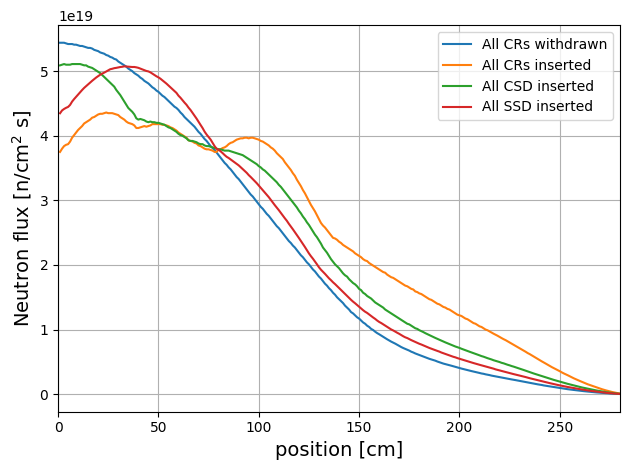
\includegraphics[width=\textwidth]{totalflux.png}
	\vspace{-0.5in}
	\caption{Radial neutron flux distribution at the mid-core for different 
	CR positions (CRs made of B$_4$C-90).} 
	\label{fig:totalflux}
\end{figure}
 

\subsubsection{Integral and differential CRW}

The integral and differential CRWs are calculated for three 
different systems: all CRs, CSD, and SSD systems. The CRs are 
inserted gradually into the core from the top to the bottom. 
Equations~\ref{Equ:4} and~\ref{Equ:5} are used to calculate the integral and 
differential CRW, respectively. Figure~\ref{fig:integ} illustrates the integral CRW for CRs 
made of B$_4$C-90. The maximum integral worth of all CRs, CSD, and SSD 
clusters are about $48.39$ $\$$, $25.30$ $\$$, and $16.46$ $\$$, respectively. The 
integral worth of SSD clusters made of B$_4$C-90 is sufficient to shut down the reactor from any 
state.

The differential CRWs are demonstrated in Figure~\ref{fig:diff}. Ideally, at the top of the core, the CR insertion has little effect since this region has low thermal neutron flux. Thus, the differential CRW has the lowest values in this region. The effect of CR insertion increases gradually near the center of the core. At the center of the core (region with maximum thermal neutron flux), the differential CRW is the largest and changes slowly with rod insertion. From the center of the core to the bottom, the differential CRW values decrease (region with low thermal neutron flux). Figure~\ref{fig:diff} shows that the maximum differential CRW is shifted toward the bottom of the core and the curves are not exactly symmetrical. This is due to the asymmetrical distribution of the fuel and graphite in simulation \cite{xuemei2013study,son2016control}.

Figure~\ref{fig:CSD} shows the integral CRW for only Control Safety Devices (CSD) clusters with six 
different absorbing materials. The results show that all absorbing materials 
have almost the same integral rod worth in the upper half of the core 
($<250$ cm from the upper boundary of the core). Further insertion of the 
CRs demonstrates that the strongest absorber, B$_4$C-90 outperforms other materials.
Notably, all results are based on steady state calculations. 

\begin{figure}
	\centering
	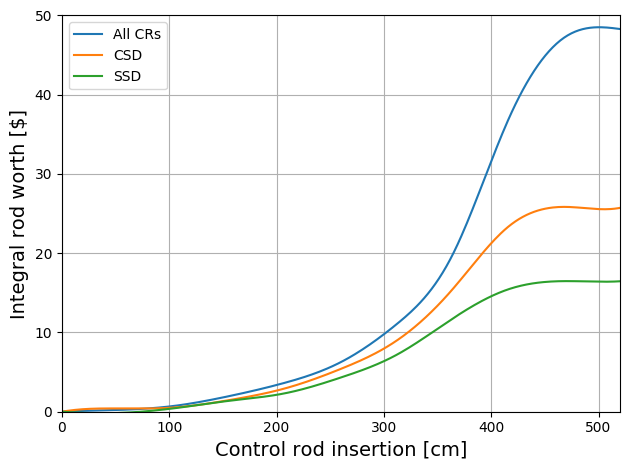
\includegraphics[width=\textwidth]{integ.png}
	\vspace{-0.5in}
	\caption{Integral CRW of all CRs, CSD, and SSD clusters (CRs made of B$_4$C-90).} 
	\label{fig:integ}
\end{figure}
\begin{figure}
	\centering
	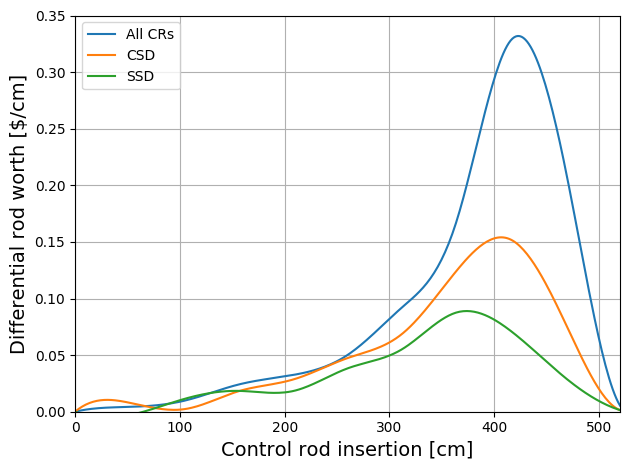
\includegraphics[width=\textwidth]{diff.png}
	\vspace{-0.5in}
	\caption{Differential CRW of all CRs, CSD, and SSD clusters (CRs made of B$_4$C-90).} 
	\label{fig:diff}
\end{figure}
\begin{figure}
	\centering
	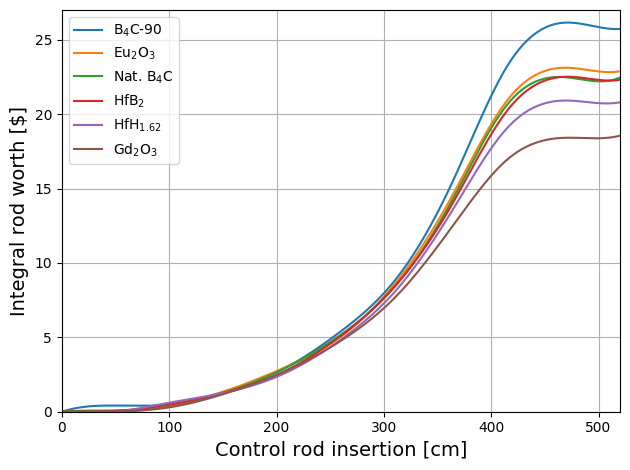
\includegraphics[width=\textwidth]{CSD.png}
	\vspace{-0.5in}
	\caption{Integral CRW of CSD clusters for various absorbing materials.} 
	\label{fig:CSD}
\end{figure}